The Silicon Photomultiplier (SiPM) is a kind of photosensor, based on semiconductor materials, developed in recent years. SiPMs are replacing progresively conventional PMTs in many experiments and applications. They archieve outstading photon-counting capabilities with higher photodetection efficiency than PMT and similar gain. SiPMs have conveninent characteristics as insensitiveness to magnetic fields, low operating voltage and compactness. The main problem with the SiPMs is their high dark count rate (between $100~\kilo\hertz$ and $1~\mega\hertz$).

SiPMs are formed by a matrix of APDs conected in parallel which are photodiodes operating in Geiger mode. APDs, the scheme of which is shown in Figure \ref{fig:SchemeAPD}, are based on p-n junctions\footnote{A p-n junction is a junction of a p+ and n+ layer, which are a tetravalent material doped with a trivalent or pentavalent material respectively, creating sublevels in the forbidden energy gap.} made with special techniques to archieve a good contact between both surfaces.(

\begin{figure}[htbp]
\centering
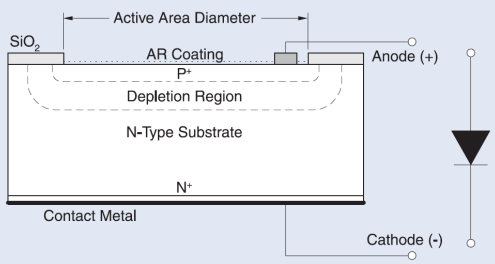
\includegraphics[scale=0.6]{3DesignPrinciples/32Tritium_detector/APD_scheme.png}
\caption{Scheme of a APD and electrical symbol used\label{fig:SchemeAPD}~\cite{OSI}.}
\end{figure}
 

The voltage at which the SiPM starts operating in Geiger mode is called the breakdown voltage, $V_ {BD}$. At lower voltages, SiPMs work in proportional mode in which the signal of the pixel is proportional to the energy deposited but their gain is lower than in Geiger mode. The experimental measurement of the breakdown voltage, described in section \ref{sec:CharacterizationSiPM}, is an important measurement to characterize a SiPM, since many properties of SiPMs depend on the overvoltage, $V_{ov}$. The overvoltage is the voltage applied to the SiPM above their own breakdown voltage and this is expressed as:

\begin{equation}
V_{bias}=V_{BD}+V_{OV}
\label{overvoltage}
\end{equation}

These APDs, called pixels when they are part of a SiPM, are connected in parallel and the sum of all of them is read. The output signal of an individual pixel is quite similar regardless of the energy deposited, with some difference because of the uncertainty due to the SiPM manufacturing process and the statistical nature of the detection process. Therefore, the energy deposited in each APD is not known but the charge of the output signal when $n$ pixels are simultaneously fired is $n$ times the charge of a single pixel, as can be checked in Figure \ref{fig:PulsesOfSiPM}. Due to this property, considering that each pixel only detects one photon, the number of detected photons is linearly proportional to the value of the output signal. Hence, after a correct calibration of SiPMs, described in section \ref{sec:CharacterizationSiPM}, the linearity of the SiPM output signal versus the deposited energy of tritium events is recovered.

\begin{figure}[h]
\centering
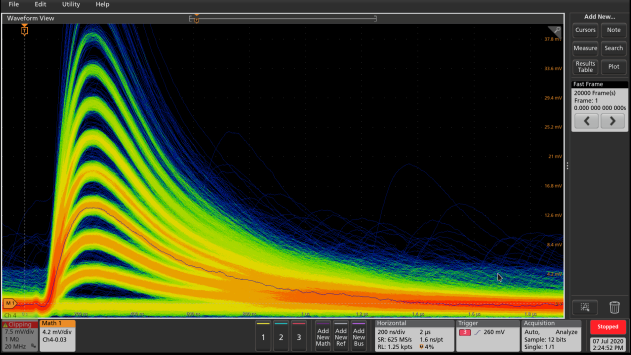
\includegraphics[scale=0.6]{3DesignPrinciples/32Tritium_detector/Several_SiPM_pulses.png}
\caption{SiPM output pulses displayed on oscilloscope, model MSO44X from Tektronix \cite{Oscilloscope}. To easily observe several heights of these pulses, associated with a different number of  SiPM pixels fired at the same time, the persistence function of the oscilloscope is used.\label{fig:PulsesOfSiPM}}
\end{figure}

The size of a SiPM pixel should be very small\footnote{Pixel sizes for commercial SiPMs are $25$, $50$ or $75\mu\meter$ \cite{DataSheetHammamatsu_1_SiPM_25}, \cite{DataSheetHammamatsu_1_SiPM_50}, \cite{DataSheetHammamatsu_1_SiPM_75}} to make sure that, for low enough photon fluxes, only one photon is detected in each pixel. If the photon flux is high (typically several thousand of photons per event) more than one photon will impinge on the same pixel, but the output signal would be that of one detected photon. This effect, known as saturation, produces a loss of linearity of the output signal. However, this effect is not important for the TRITIUM detector since its scintillating signals are far from producing so many photons. %The experimental measurements of this effect, which have been done for our SiPMs, is shown in section \ref{sec:CharacterizationSiPM}. 

The SiPM can be modeled as an electric circuit, shown in figure \ref{subfig:ElectricModelSiPM}, in which, due to the charge distribution in the depletion zone, a capacitance is induced by the SiPM. This looks like a reverse diode in parallel with a capacitor of capacitance $C_d$. When the pixel detects a photon, the capacitor is discharged, creating an output current (electronic pulse).

In addition, each pixel of a SiPM has a quenching resistance\footnote{The tipical valuer of this quenching resistance for commercial SiPMs is around $500~\kilo\Omega$} in serie, $R_q$, that stops the current produced when this pixel is fired. When the discharge is produced, a current flows through the resistance, reducing the reverse voltage seen by the diode below the breakdown voltage. Then, the current that flows through the diode is stopped and the voltage seen by the diode is reset to the bias voltage. This pixel is ready to detect a new photon again. This behaviour is schematicaly shown in Figure \ref{subfig:HowSiPMworks}.

\begin{figure}
\centering
    \begin{subfigure}[b]{0.45\textwidth}
    \centering
    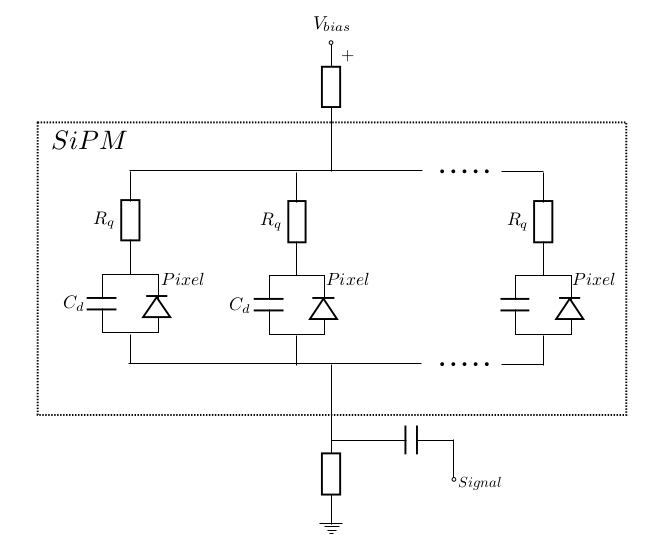
\includegraphics[width=\textwidth]{3DesignPrinciples/32Tritium_detector/SimpliestElectronicSchemeSiPM.png}  
    \caption{\label{subfig:ElectricModelSiPM}}
    \end{subfigure}
    \hfill
    \begin{subfigure}[b]{0.45\textwidth}
    \centering
    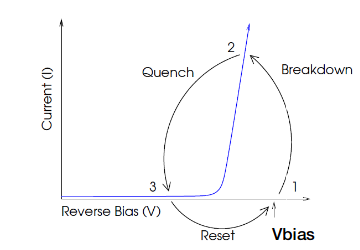
\includegraphics[width=\textwidth]{3DesignPrinciples/32Tritium_detector/How_a_quenching_resistence_in_a_SiPM_works.png}  
    \caption{\label{subfig:HowSiPMworks}}
    \end{subfigure}
 \caption{(Left) Electronic scheme of a SiPM and (right) output current of a SiPM as a function of the reverse voltage. It is seem that the quenching mechanism is essential for working with SiPMs~\cite{DataSheetSensL}.}
 \label{fig:ChenchingResistance}
\end{figure}

The recovery of the bias voltage seen by the SiPM after photon detection is characteristic of a RC circuit, described by the equation: 

\begin{equation}
V_{bias}(t)=V(t_0)\left(1-e^{-t/\tau} \right)
\label{RCCircuitBiasVoltage}
\end{equation}
where $\tau$ is the recovery time constant of the system, given by $\tau=C_d \times R_q$. In section \ref{sec:CharacterizationSiPM} the capacitance $C_d$ and the quenching resistance $R_q$ are experimentally measured and the recovery time constant extrapolated from both.

SiPM gain (typically of the order of $10^6$) is defined as the charge produced when a single pixel is fired. This can be measured experimentally from its Single Photon Spectrum, SPS, which is the spectrum obtained when the SiPM output signal is integrated (charge) and histogrammed. The experimental measurement of the SPS and the calculation of the gain is presented in section \ref{sec:CharacterizationSiPM}. It has to be taken into account that the SiPM gain is highly dependent on temperature, which cannot be controlled with sufficient sensitivity (less than $1\celsius$) in the final emplacement of the TRITIUM monitor. Therefore, a gain stabilization method was developed to compensate for the temperature effect. This method is detailed in section \ref{sec:CharacterizationSiPM}.

An important parameter for the SiPM used in the TRITIUM project is the photon detection efficiency, PDE. This is defined as the probability of recording the electrical pulse produced by a photon that hit the SiPM. The PDE of a SiPM consists of a product of three different paramenters, the fill factor ($FF$), which is the ratio between the active area of the SiPM and the total area, the quantum efficiency for photoelectron conversion ($QE$), which is the probability that a incident photon generate an electron-hole pair, and the probability that the generated electron or hole produces an avalanche, $P_{av}$.

\begin{equation}
PDE=FF \times QE \times P_{av}
\label{PDE_SiPM}
\end{equation}

Like PMTs, sometimes the SiPM produces pulses that are unrelated with any incident photon. The current due to these pulses is called the dark current rate. It depends on temperature. At temperatures around $25\celsius$, these pulses are mainly produced by the thermal generation, i.e., when a free electron or hole start an avalanche. The dark current signal is identical to the signal produced by a single photon, so they cannot be discriminated. Therefore, it is very important to determine the importance of the dark current on the tritium signal.

Electrons contained in an avalanche of a SiPM pixel emit secondary optical photons\footnote{Around 20 secondary optical photons are emitted in each SiPM output pulse with gains of the order of $10^6$ \cite{CrosstalkProbability}}. These optical photons can reach other pixels, producing new avalanches. This effect, called optical crosstalk, produces signals that are larger than those corresponding to single photons, producing erroneous information about the number of photons detected. The probability of producing an optical crosstalk event depends on the number of electrons produced in the avalanche (gain) and, therefore, on the temperature and the overvoltage. This probability at the recommended overvoltage and temperatures around $25\celsius$ is typically less than $10\%$.

The PED, dark count rate and crosstalk are not experimentaly measured yet since a different setup, shown in reference \cite{PDEStudy}, is needed. These parameters will be measured for the SiPM model used in the final version of TRITIUM monitor.

Due to imperfections existing in the cristal lattice of a SiPM, called traps, an electron of an avalanche can be captured and released after a characteristic time, $\tau_t$. If this characteristic time is longer than the time used to recover the charge of the pixel, typically $3\tau$, this electron can trigger a new avalanche which will be seen as a new event. This events, called  afterpulses, are often emitted around $1~\mu\second$ after SiPM output pulses. The afterpulse probability was not measured since it is not interesting for the TRITIUM project. The reason is that the TRITIUM detector uses the SiPM as a counter (without integrating the signal). In addition, time coincidences are made using time windows of $10~\nano\second$. At this level, the afterpulse probability is negligible since it normally happen $1~\mu\second$ after the SiPM output pulse.

The initial SiPM cadidate for TRITIUM project and the one which was characterized is the model S13360-1375 from Hamamatsu Photonics \cite{DataSheetHammamatsu_1_SiPM_1375} because this model has interesting characteristics and properties, shown in Table \ref{tab:PropertiesOfSiPM1375}. This model was mainly choosen due to its large pixel size, $75~\mu\meter$, which implies a high PDE and a high gain, both important parameters for the TRITIUM project due to the low activity to be detected and to the small signals produced by tritium events. High PDE and high gain are achieved at the cost of reducing the dinamic range, which is not an issue due to the small signals generated by tritium events. 

\begin{table}[htbp]
\centering{}%
\begin{tabular}{lcc}
\toprule 
Parameter & S13360-1375 & S13360-6075 \tabularnewline
\midrule
\midrule 
Series & $S13360$ & $S13360$ \tabularnewline
Model & $1375$ & $16075$ \tabularnewline
Pixel Pitch ($\mu\meter$) & $75$ & $75$ \tabularnewline
Effective photosensitive area ($\mm^2$) & $1.3 \times 1.3$ & $6.0 \times 6.0$ \tabularnewline
Number of pixels & $285$ & $6400$ \tabularnewline
Fill factor & $82\%$ & $82\%$ \tabularnewline
Refractive index of windows material & $1.55$ & $1.55$ \tabularnewline
Operating temperature range ($\celsius$) & $[-20,60]$ & $[-20,60]$ \tabularnewline
Spectral response range, $\lambda$ ($\nano\meter$) & $[320, 900]$ & $[320, 900]$ \tabularnewline
Peak sensitivity wavelength, $\lambda_p$ ($\nano\meter$) & $450$ & $450$ \tabularnewline
PhotoDetection Efficiency, PDE, $\lambda=\lambda_p$ ($\%$) & $50$ & $50$ \tabularnewline
Dark counts, Typical/Maximum (kcps) & $90/270$ & $2000/6000$ \tabularnewline
Terminal capacitance, $C_t$ ($\pico\farad$) & $60$ & $1280$ \tabularnewline
Gain, M, & $4 \cdot{} 10^6$ & $4 \cdot{} 10^6$ \tabularnewline
Breakdown Voltage, $V_{BD}$ ($\volt$) & $50.97$ & $53$ \tabularnewline
Cross talk probability($\%$) & $7$ & $7$ \tabularnewline
Temperature coefficient $\Delta TV_{op}$ (m$\volt/\celsius$) & $54$ & $54$ \tabularnewline
\bottomrule
\end{tabular}
\caption{Characteristics of SiPM S13360-1375 and S13360-6075 from Hamamatsu Photonics \cite{DataSheetHammamatsu_1_SiPM_1375}.}
\label{tab:PropertiesOfSiPM1375}
\end{table}

These parameters quoted in Table \ref{tab:PropertiesOfSiPM1375}, provided by Hamamatsu photonics, are only an approximation for a given element. They can vary significatively even for SiPMs of the same model, so they must be measured for each SiPM used. The measurement of some important characteristics for the TRITIUM project is reported in section \ref{sec:CharacterizationSiPM}. 

This SiPM was also chosen because, as it can be observed in Figure \ref{fig:PDESiPM}, its maximum PDE is reached at $\lambda_{p,SiPM}=450~\nano\meter$, which is very close to the peak of the emission spectrum of the scintillating fibers used, $\lambda_{p,fiber}=435~\nano\meter$.

\begin{figure}[htbp]
\centering
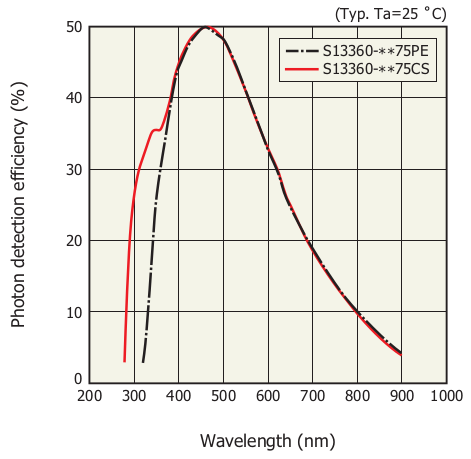
\includegraphics[scale=0.6]{3DesignPrinciples/32Tritium_detector/SiPMPDE.png}
\caption{Photon detection efficiency (PDE) spectrum for SiPM S13360-**75 models~\cite{DataSheetHammamatsu_1_SiPM_1375}.\label{fig:PDESiPM}}
\end{figure}

This SiPM was later replaced by the more performant model S13360-6075 from Hamamatsu Photonics \cite{DataSheetHammamatsu_1_SiPM_75}, whose properties are also listed in Table \ref{tab:PropertiesOfSiPM1375}. The only difference between both models is their active area ($6\times6~\mm^2$) that allow to read more scintillating fibers with the second model. This improvement is achieved at the price of a higher dark count rate (typically 2 Mcps). In addition, commercial matrices are available, with a total area of $24\times24~\mm^2$.

Although TRITIUM detector uses whole SiPM matrices, the caracterization has been carried out at the level of a single SiPM to learn about the values of the SiPM parameters and to test the gain control method. A new experimental setup, detailed in appendix \ref{App:ElectronicReadoutSiPM}, is already  prepared to perform a complete characterization of the SiPM model S13360-6075.